% Figure 1: Inside-Out Evolution Model
\documentclass[tikz,border=10pt]{standalone}
\usepackage{tikz}
\usetikzlibrary{arrows.meta,positioning,shapes,calc,decorations.pathreplacing,fit,backgrounds,patterns}

\begin{document}
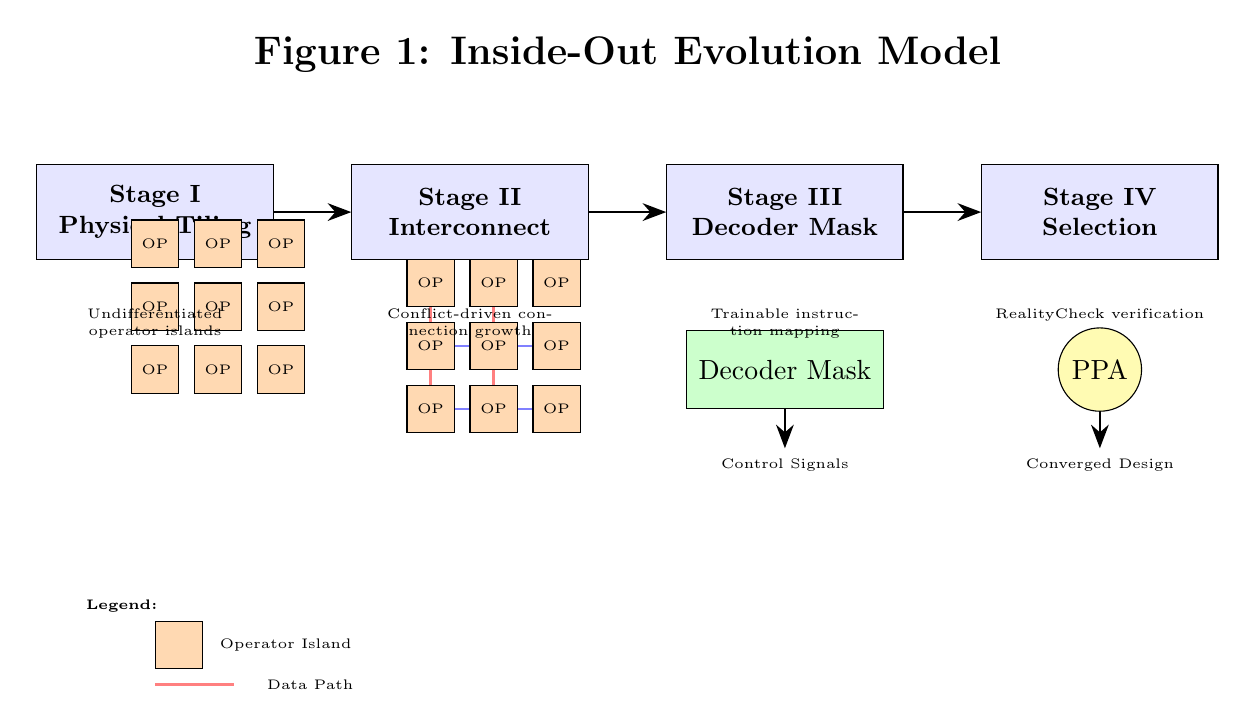
\begin{tikzpicture}[
    node distance=1.5cm and 2cm,
    box/.style={rectangle, draw, minimum width=2.5cm, minimum height=1cm, align=center, font=\small},
    stage/.style={rectangle, draw, fill=blue!10, minimum width=3cm, minimum height=1.2cm, align=center, font=\small\bfseries},
    operator/.style={rectangle, draw, fill=orange!30, minimum size=0.6cm, font=\tiny},
    arrow/.style={-{Stealth[length=3mm]}, thick}
]

% Title
\node[font=\Large\bfseries] at (0,6) {Figure 1: Inside-Out Evolution Model};

% Stage I: Physical Tiling
\node[stage] (s1) at (-6,4) {Stage I\\Physical Tiling};
\begin{scope}[shift={(-6,2)}]
    \foreach \x in {0,1,2} {
        \foreach \y in {0,1,2} {
            \node[operator] at (\x*0.8,\y*0.8) {OP};
        }
    }
\end{scope}
\node[below=0.5cm of s1, font=\tiny, text width=3cm, align=center] {Undifferentiated operator islands};

% Stage II: Self-Organizing Interconnect
\node[stage] (s2) at (-2,4) {Stage II\\Interconnect};
\begin{scope}[shift={(-2.5,1.5)}]
    \foreach \x in {0,1,2} {
        \foreach \y in {0,1,2} {
            \node[operator] (op\x\y) at (\x*0.8,\y*0.8) {OP};
        }
    }
    \draw[thick,red!50] (op00) -- (op01) -- (op02);
    \draw[thick,red!50] (op10) -- (op11) -- (op12);
    \draw[thick,blue!50] (op00) -- (op10) -- (op20);
    \draw[thick,blue!50] (op01) -- (op11) -- (op21);
\end{scope}
\node[below=0.5cm of s2, font=\tiny, text width=3cm, align=center] {Conflict-driven connection growth};

% Stage III: Functional Differentiation
\node[stage] (s3) at (2,4) {Stage III\\Decoder Mask};
\node[rectangle, draw, fill=green!20, minimum width=2.5cm, minimum height=1cm] (dm) at (2,2) {Decoder Mask};
\draw[arrow] (dm) -- ++(0,-1) node[below, font=\tiny] {Control Signals};
\node[below=0.5cm of s3, font=\tiny, text width=3cm, align=center] {Trainable instruction mapping};

% Stage IV: Environmental Selection
\node[stage] (s4) at (6,4) {Stage IV\\Selection};
\node[circle, draw, fill=yellow!30, minimum size=1cm] (ppa) at (6,2) {PPA};
\draw[arrow] (ppa) -- ++(0,-1) node[below, font=\tiny] {Converged Design};
\node[below=0.5cm of s4, font=\tiny, text width=3cm, align=center] {RealityCheck verification};

% Arrows between stages
\draw[arrow] (s1) -- (s2);
\draw[arrow] (s2) -- (s3);
\draw[arrow] (s3) -- (s4);

% Legend
\node[anchor=west, font=\tiny] at (-7,-1) {\textbf{Legend:}};
\node[operator, anchor=west] at (-6,-1.5) {};
\node[anchor=west, font=\tiny] at (-5.3,-1.5) {Operator Island};
\draw[thick,red!50, anchor=west] (-6,-2) -- (-5,-2);
\node[anchor=west, font=\tiny] at (-4.7,-2) {Data Path};

\end{tikzpicture}
\end{document}
